\documentclass[10pt]{scrartcl} % use larger type; default would be 10pt

\usepackage[utf8]{inputenc} % set input encoding (not needed with XeLaTeX)
\usepackage[cm]{fullpage}
\usepackage{amsmath}
\usepackage{caption}
\usepackage{float}
\usepackage{graphicx} % support the \includegraphics command and options
\usepackage{biblatex} % use biber command to regenerate references
\usepackage{subcaption}

\renewcommand{\bibfont}{\footnotesize}
%\pagenumbering{gobble}
\usepackage{hyperref}
\addbibresource{report.bib}

\title{Accurate Vision-Based Landing For Multicopter UAVs}
\subtitle{CS287: Project Report}
\author{Constantin Berzan, Sunil Shah}
\date{} 

\begin{document}
\maketitle

\begin{abstract}
Multicopter UAVs have become increasingly popular over the last five years and are being considered for commercial purposes. However, they are hampered by their limited battery life. This class project is part of a larger project to build an automatic charging station for multicopters. Currently openly available automated landing algorithms rely on GPS to localise the UAV with respect to the landing station. We show that this approach is considerably inaccurate and implement a vision-based landing system which uses pose estimates to more accurately localise the UAV. 
In order to land based on this data, we build a state machine and controller that interacts with the open source ArduCopter autopilot to bring a test quadcopter down to a landing pattern. While environmental conditions and hardware issues ultimately prevented us from realising a vision-based landing, we are confident that, in good conditions and with some slight modification, our system should be able to land with much greater accuracy than GPS.
\end{abstract}
%%%%%%%%%%%%%%%%%%%%%%%%%%%%%%%%%%%%%%%%%%%%%%%%%%%%%%%%%%%%%%%%%%%%%%%%%%%%%%
\section{Motivation}
In the recent past, multicopter UAVs (or drones, as they are colloquially known) have become increasingly popular. This has been well documented by both mainstream and technology media. Once the preserve of the military, several factors have led to multicopter UAVs being fabricated and flown by hobbyist pilots:
\begin{description}
\item[The Maker Movement]{Affordable 3D printing have made it easier to prototype and produce cheap multicopter airframes.}
\item[Commodity Embedded Electronics]{A number of projects, beginning with the Arduino platform, have made well supported embedded computers available at low cost to the general public.}
\item[Open Source Software]{There are a number of popular open source autopilot projects that have significantly lowered the barrier to entry to novice users.}
\item[Smartphone IMUs]{As smartphones have grown in popularity, it has become possible to source low cost inertial measurement units which measurement of acceleration along several axes.}
\item[Ease of Control]{Multicopter UAVs offer the vertial take off and landing versatility of a traditional rotorcraft but with increased ease of control.}
\end{description}

These factors allow UAVs to be bought off the shelf for less than a thousand dollars, which is several orders of magnitude less than the cheapest traditional UAV. As with any disruptive technology, there is growing interest in the potential commercial applications. 

However, before these craft can be used reliably in a commercial setting, there are a number of shortfalls. This project aims to address two of these:
\begin{enumerate}
\item{Multicopter craft consume a lot of power. Battery life is limited to 30 minutes for the most efficient craft with large batteries.}
\item{Autonomous landing relies on GPS for localisation. This has limited accuracy.}
\end{enumerate}

\subsection{Automated Charging}

In a commercial context, UAVs become limited by their short battery life. If a user wishes to perform a mission that takes longer than the battery life of a UAV, they have to operate multiple UAVs and be response for battery handling (which typically involves removing a battery, plugging it into specialised equipment for at 30-60 minutes). This adds to the operational complexity and ultimately the cost for operating UAVs.

% TODO: Add references
One approach to mitigating the short battery life of a UAV is to have it land on a charging station. 

\subsubsection{Inductive Charging}
Several approaches have used inductive charging, where an oscillating magnetic field in the base of the charging station induces current in a coil on the UAV and charges the battery. While this approach allows for considerable inaccuracy in landing, it is approximately 20x slower than conductive charging and requires extra equipment on the UAV itself which impedes its aerodynamic efficiency.

\subsubsection{Conductive Charging}
A more traditional approach is to consider conductive charging. This is extremely efficient and offers very fast charge times. Additionally, it requires minimal modification to the airframe itself. However, contacts have to be positioned very accurately. As part of an ongoing Master's capstone project, we have designed a mechanically actuated charging station that uses an arm to bring a UAV into charging contacts (Fig \ref{fig:catia}). 

This approach requires accurate landing of the UAV onto a predefined area of the charging station.

\begin{figure*}[h]
    \centering
    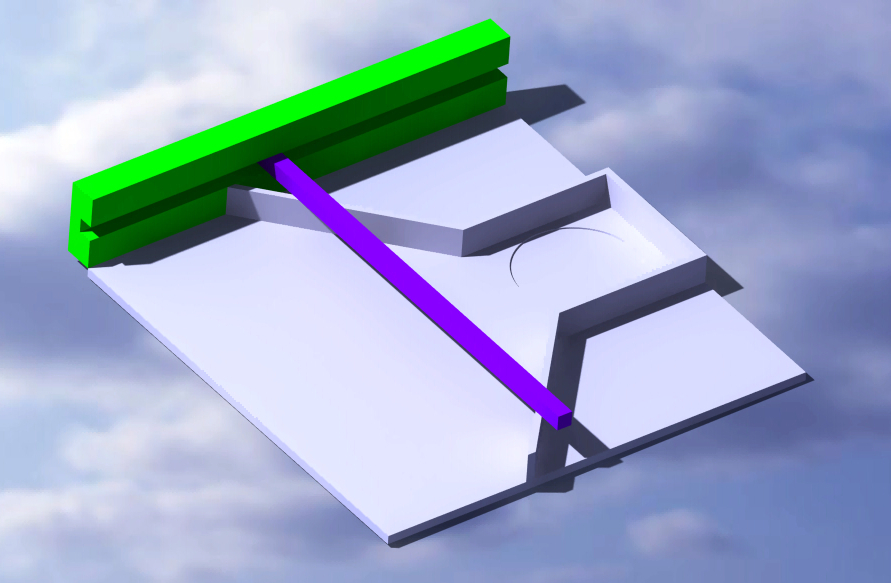
\includegraphics[width=\textwidth]{images/catia.jpg}
    \caption{Our design for a UAV charging station.}
    \label{fig:catia}
\end{figure*}


\subsection{Accurate Landing}

%% SUNIL
%% What is the problem? Why does it matter?



% Delivery
% The automated problem also becomes relevant for when UAVs are used for delivery
% 

% Current solutions use GPS to localise, which tracks accuracy of GPS.
% Vision based approaches yield considerably better accuracy but are not available

% Our project was to make such an implementation available that ran on 
% commodity drones and hardware.


\begin{figure*}[h]
    \centering
    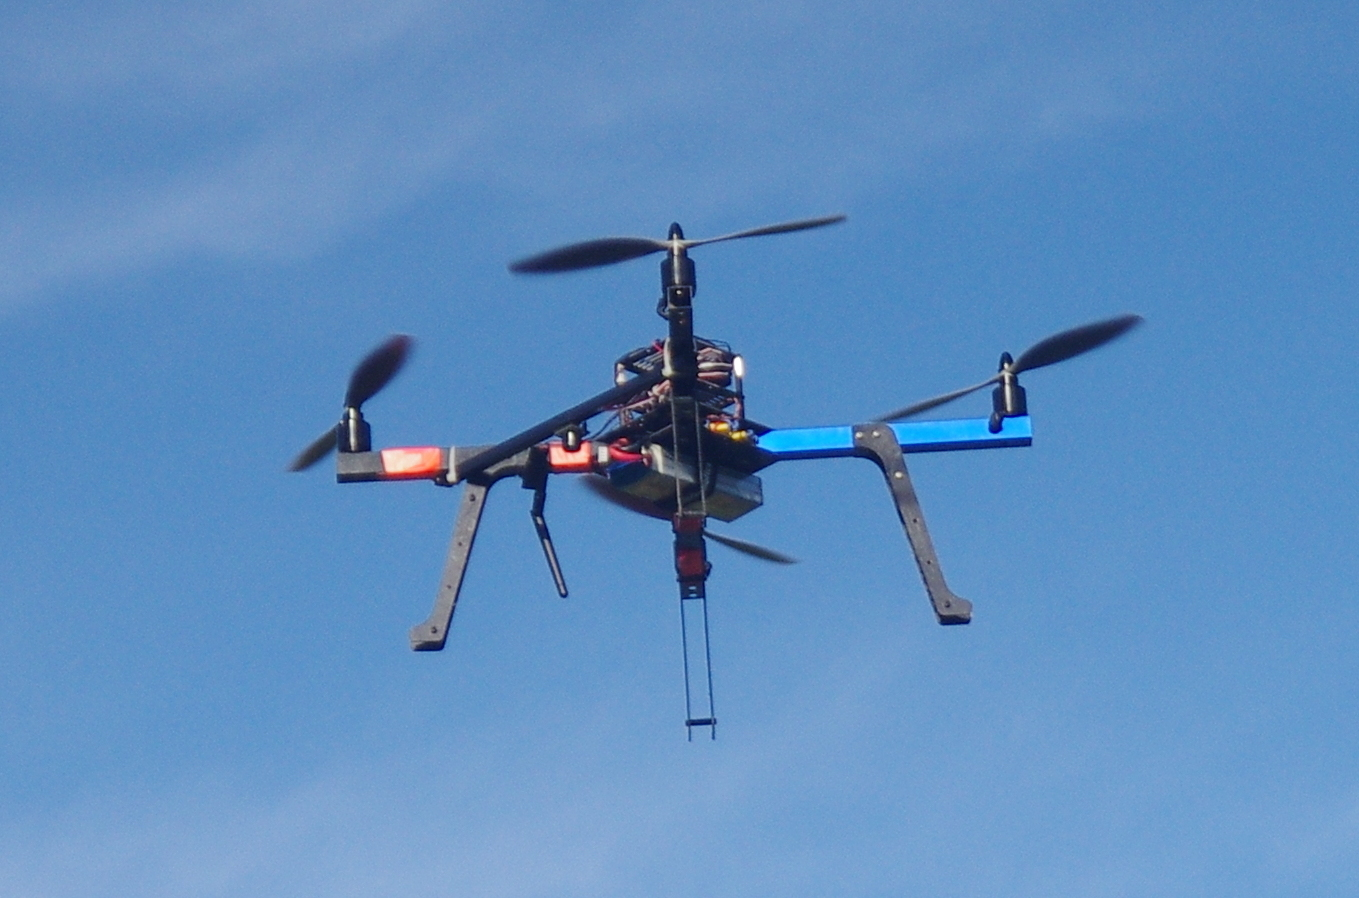
\includegraphics[width=\textwidth]{images/drone.jpg}
    \caption{Our test quadcopter in action.}
    \label{fig:drone}
\end{figure*}


\section{Prior Work}

The automated landing problem has been investigated in the research literature
of the early 2000s. Here we briefly describe the approaches taken by some of
the most cited papers on this topic.

Sharp, Shakernia, and Sastry \cite{sharp_et_al_2001} designed an approach for
automatically landing an unmanned helicopter. Their landing target uses a
simple monochromatic design made up of several squares. Onboard the helicopter,
they use a pan-tilt-zoom camera and two embedded computers with Intel CPUs.
They discuss the details of their approach to pose estimation, but omit the
details of the helicopter controller. Using a real-time OS and optimized custom
code, they are able to get their vision system to operate at a rate of 30 Hz.

Our own approach in this project is modeled after that of Sharp et al. The main
differences are that (1) we use cheap off-the-shelf hardware, rather than
research-grade hardware; (2) our camera is stationary, it is not capable of
panning or tilting; and (3) we use off-the-shelf software components such as
ROS and OpenCV, rather than writing all of our code from scratch.

Saripalli, Montgomery, and Sukhatme \cite{saripalli_et_al_2002} designed
another approach for automatically landing an unmanned helicopter. They use a
monochromatic H-shaped landing target. Their onboard vision system detects this
landing target and outputs the helicopter's relative position with respect to
it. This is sent wirelessly to a behavior-based controller running on a ground
station, which then directs the helicopter to land on top of the target. They
are able to run their controller at 10 Hz this way. They are also using a
high-accuracy differential GPS system, and it is not clear how much their
differential GPS and vision systems contribute to a successful landing.

Garcia-Pardo, Sukhatme, and Montgomery \cite{garcia_pardo_et_al_2002} look at a
more general problem, where there is no pre-specified landing target, and their
helicopter has to search autonomously for a suitable clear area on which to
land.


\section{Approach}

\subsection{Architecture}

\begin{figure}[h!]
    \centering
    \begin{subfigure}[b]{0.9\textwidth}
        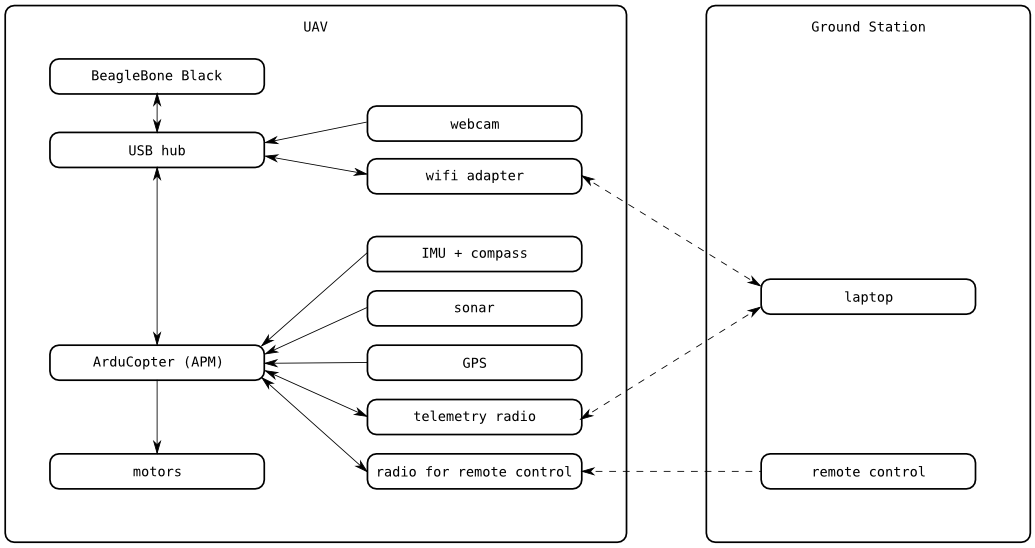
\includegraphics[width=\textwidth]{images/architecture.png}
        \caption{
            Architecture of our automated landing system. We use inexpensive
            off-the-shelf hardware. The laptop and remote control are for
            monitoring and emergency takeover by a human pilot. All the
            computation is performed onboard the UAV.
        }
    \end{subfigure}
    \\~\\
    \begin{subfigure}[b]{0.9\textwidth}
        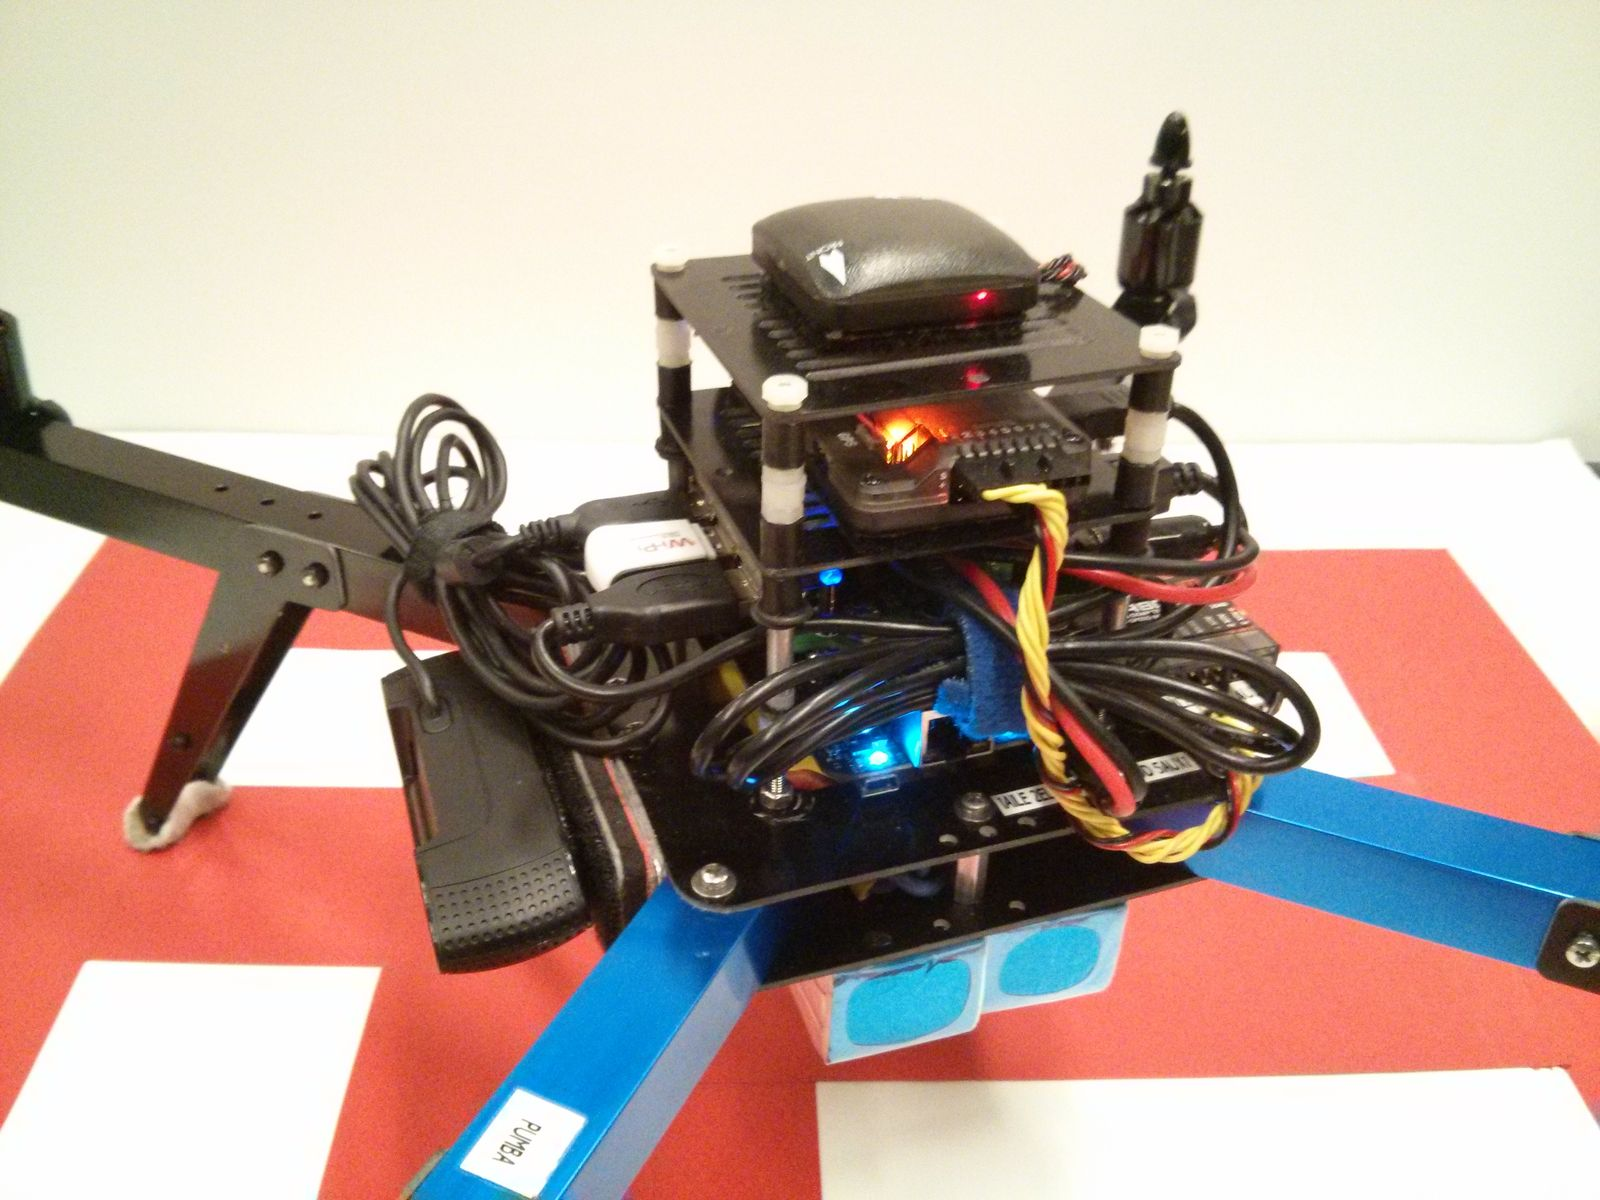
\includegraphics[width=\textwidth]{images/hardware.jpg}
        \caption{
            Our hardware stack fully assembled. From bottom to top: batteries,
            BeagleBone embedded computer, USB hub with Wi-Fi adapter, 3D
            Robotics autopilot (APM) with embedded sensors, GPS module. The
            webcam is on the left, and the radio for the remote control is on
            the right.
        }
    \end{subfigure}
    \caption{Hardware architecture and setup}
    \label{fig:hardware}
\end{figure}

Our goal was to use inexpensive, off-the-shelf hardware, rather than expensive
equipment that is only accessible to researchers. We used quadcopter components
made by 3D Robotics, together with their ArduCopter autopilot (frequently
referred to under its old name -- Ardu-Pilot Mega, or APM) and associated GPS
module. This autopilot acts as a low-level controller that keeps the quadcopter
stable. It runs an unmodified version of the open-source autopilot code
provided by 3D Robotics.

We augmented the quadcopter with a BeagleBone Black embedded computer, which
uses a 1 GHz ARM CPU. (Since the ARM architecture is so different from x86,
the 1 GHz figure should not be compared to the frequency of modern-day Intel
CPUs, which are far more advanced, and expensive.) Using a powered USB hub, we
connected the autopilot to the BeagleBone. We also connected the webcam and a
Wi-Fi adapter this way.

% TODO:
% Weight of hardware stack?
% Estimated power consumption?
% Estimated cost of system?

On the BeagleBone, we installed a pre-built image of the Ubuntu 12.04
distribution, obtained from {\tt armhf.com}. We installed pre-built packages
for ROS groovy from the official ROS repositories. We compiled OpenCV 2.4.7 by
hand. We also installed roscopter, a third-party piece of software that reads
the state of the autopilot and makes it available via ROS, and also makes it
possible to send controls to the autopilot.


\subsection{Vision}
%% NAHUSH 
% Describe the vision approach we took

\subsubsection{Corner Detection}
%% NAHUSH

\begin{figure*}[h]
    \centering
    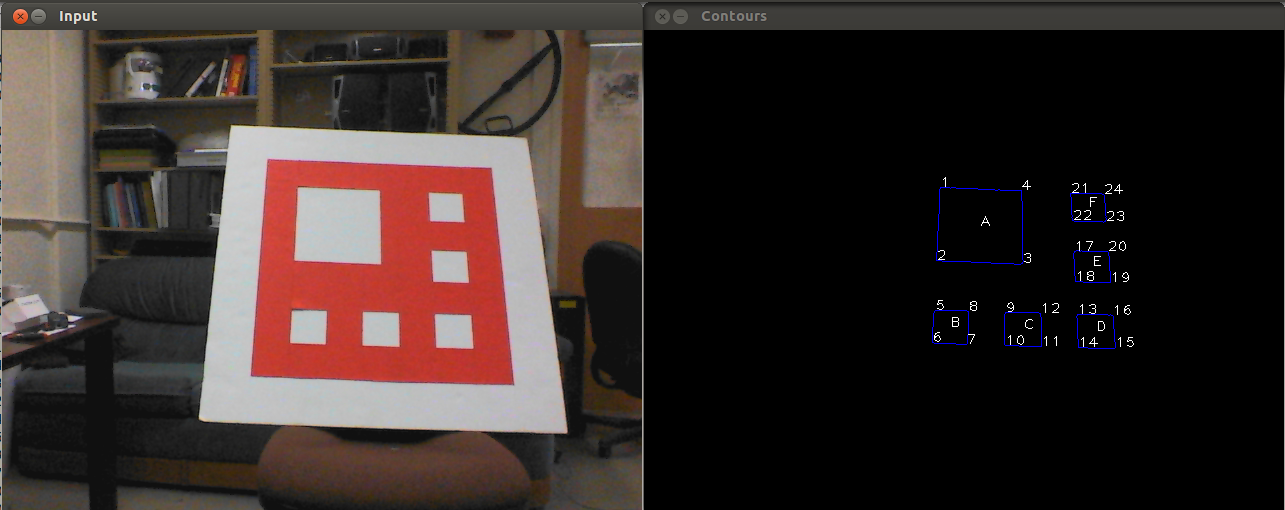
\includegraphics[width=\textwidth]{images/corners.png}
    \caption{Corner detection in action.}
    \label{fig:corners}
\end{figure*}

\subsubsection{Pose Estimation}

We define the origin of the world coordinate frame to be the center of the
landing platform, such that all points on the landing platform have a Z
coordinate of zero. The corner detector gives us image coordinates for the 24
corners. Thus, we have a set of 24 point correspondences between world
coordinates and image coordinates. Given this input, we want to compute the
quadcopter's pose, i.e. the position and orientation of the camera in the world
coordinate frame. To do this, we follow the approach of Sharp et al.
\cite{sharp_et_al_2001}.

% TODO: show math
% Have 48 equations (2 for each point pair)
% System of equations has 6 degrees of freedom

The output from the pose estimator is a translation vector
$t = \begin{bmatrix} t_x & t_y & t_z \end{bmatrix}^\top$
and a 3x3 rotation matrix $R$. We compute the camera position in world
coordinates as $C = -R^\top t$, and the yaw angle as
$\alpha = \arctan(R_{21} / R_{11})$. (The roll and pitch angles can be computed
similarly, but we do not require them in the control algorithm.)

The approach above assumes a calibrated pinhole camera. For the pose estimates
to be meaningful, our camera had to be calibrated first. We calibrated our
camera using the {\tt camera\_calibration} tool provided in the OpenCV
tutorials, plus some manual tuning. We used the resulting calibration matrix to
convert the raw pixel coordinates into coordinates for a calibrated pinhole
camera model, which we then fed into the equations above.


\subsection{Control}
%% SUNIl

In order to actually land our UAV using our pose estimates, it was necessary to implement a landing controller. Since this would need to run in real time (in order to adequately stabilise the UAV), we deferred real-time control to the \textit{loiter} mode provided by the ArduCopter autopilot. This takes care of real-time stabilisation for us and, additionally, attempts to keep the UAV in the same location using GPS. (They also offer a more basic stabilise mode which doesn't attempt to keep the craft to one location.)

Using the roscopter library, we were able to override the radio control inputs that would typically be received from the user. Using these inputs, we could manipulate the throttle, yaw, pitch and roll of the UAV.

\subsubsection{State Machine}
We designed a state machine with five states, beginning in a \textit{FLYING} mode and ending in \textit{POWER\_OFF}. Fig \ref{fig:statediagram} shows the transitions between the states. 

\paragraph{FLYING}
The \textit{FLYING} state represents when the UAV is not under our control, for instance, when the user is in manual control or has invoked another autopilot mode. Our controller listens to a specific channel of the radio input which represents three fixed values that are user selectable on the handheld transmitter. When the value of that channel changes to a predefined value, our controller takes control of the autopilot and transitions into \textit{SEEK\_HOME}.

\paragraph{SEEK\_HOME}
In \textit{SEEK\_HOME} mode, we use the built in \textit{return to launch} mode that ArduCopter implements - this navigates the UAV back to the launch location. Once above the launch location, the UAV should start receiving valid pose estimates.

\paragraph{LAND\_HIGH}
Our controller enters the \textit{LAND\_HIGH} mode when it starts receiving valid pose estimates. We use a simple proportional controller to calculate the appropriate control inputs based on the deviation from the centre of the landing station (in terms of x, y and yaw). These comprise the error terms in our controller.

Our controller disregards the z deviation and descends at a fixed rate. The z deviation is, however, used as the best estimate of altitude (our tests, described in section SECTION, show that the calculated z value is extremely accurate). When the UAV reaches a predefined altitude (where we know pose estimates will no longer be possible, due to field of view limitations), our controller enters into the \textit{LAND\_LOW} state.

\paragraph{LAND\_LOW}
In \textit{LAND\_LOW}, we use a dead reckoning approach to the ground since we are no longer able to receive valid pose estimates. Our controller attempts to keep the UAV flying straight and level and descends at a fixed rate. It uses data from the barometric pressure sensor to determine when the UAV has reached the ground and then enters into the \textit{POWER\_OFF} state.

\paragraph{POWER\_OFF}
\textit{POWER\_OFF} retains control of the UAV but sets throttle to a low value to prevent it from flying.

\begin{figure*}[h]
    \centering
    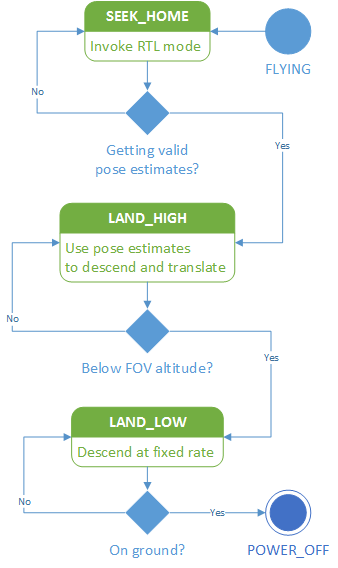
\includegraphics{images/statediagram.png}
    \caption{The state diagram of our landing controller.}
    \label{fig:statediagram}
\end{figure*}

\subsection{Software Integration}
%% SUNIL

% A brief word on ROS + diagram showing the flow of messages?

\section{Results}

\subsection{Pose Estimation Accuracy}

We tested the accuracy of our pose estimator in the lab, by holding the camera
above the landing pad, and comparing the true measured height to the height
reported by the pose estimator. We also measured the standard deviation in our
pose estimate, by taking multiple measurements of the same scene. We compared
the standard deviation on x and y to the lower bound given by the dimensions on
the ground plane that correspond to one pixel in a 640x480 image at a given
height. Table \ref{tab:pose-accu} shows these results. There is a small (1.4\%
relative) systematic overestimation of the true height. This can be corrected
by doing more precise calibration. The height estimate is very stable at these
heights (small standard deviation). The x and y estimates are also fairly
accurate, although the error in these estimates is an order of magnitude
greater than the lower bound. This is consistent with the fact that there is
some noise in the corner detection, and the pose estimator finds an approximate
solution. In summary, this experiment suggests that our pose estimates should
be good enough to reliably land our quadcopter. If individual measurements are
too noisy, it is possible to get better pose estimates using a Kalman filter,
although that requires having a model of the dynamics and controls of the
system.

\begin{table}[h!]
    \centering
    \begin{tabular}{c|cc|cc|cc|c}
        true height & z mean    & z std     & x bound   & x std     & y bound   & y std     & yaw std \\
        \hline
         88 cm      & 89.3 cm   & 0.05 cm   & 0.19 cm   & 0.43 cm   & 0.14 cm   & 0.39 cm   & 0.12 $^{\circ}$ \\
        120 cm      & 121.1 cm  & 0.08 cm   & 0.26 cm   & 1.16 cm   & 0.19 cm   & 1.06 cm   & 0.12 $^{\circ}$ \\
        170 cm      & 172.0 cm  & 0.18 cm   & 0.37 cm   & 2.74 cm   & 0.27 cm   & 2.17 cm   & 0.07 $^{\circ}$ \\
        226 cm      & 229.0 cm  & 0.54 cm   & 0.49 cm   & 6.51 cm   & 0.36 cm   & 6.05 cm   & 0.34 $^{\circ}$ \\
    \end{tabular}
    \caption{
        Accuracy of our pose estimates. ``x bound'' and ``y bound'' are lower
        bounds for the error on x and y, given by the limited image resolution.
    }
    \label{tab:pose-accu}
\end{table}

\subsection{Performance}
%% CONSTANTIN

Camera is capable of 30 FPS
Just capturing frames: 11.2 FPS
Pose estimator running: 3.0 FPS
Pose estimator and roscopter running: 1.6 FPS

% Rate our system against the system they had in 2001 which ran at near real time FPS

\subsection{Control}
%% SUNIL 
% How did our controller do?
% Field of view of camera and size of landing pad meant no accurate Z estimates
% below ~ 2m.
% Noisy sensor data = state transitions wer edifficult

\section{Challenges}
One of the significant impediments to our project was integrating working hardware. In this section, we describe the issues we had and how they might be mitigated in the future.

\subsection{Integration of Hardware}
%% CONSTANTIN
% A brief note on the hardware travails we had.

\subsection{Image Quality}
%% NAHUSH
% Mention the issue with motion blur up in the air and possible solutions (better camera with more fine grained control)

\begin{figure*}[h]
    \centering
    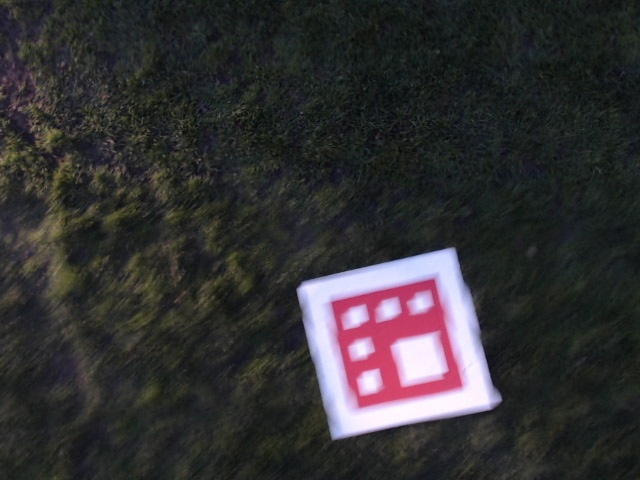
\includegraphics[width=\textwidth]{images/badimage.jpg}
    \caption{An example of a bad image.}
    \label{fig:badimage}
\end{figure*}

\subsection{Field of View}
%% NAHUSH

% Drone needs to be at 1 metre to see the landing pad.
% Practically, this means we need to be at about 2 metres to get
% pose estimates.

% height	visible land area
% 1 m	1.37 m x 0.77 m
% 2 m	2.75 m x 1.54 m
% 4 m	5.50 m x 3.07 m
% 8 m	11.0 m x 6.14 m
% 16 m	22.0 m x 12.3 m

\begin{figure*}[h]
    \centering
    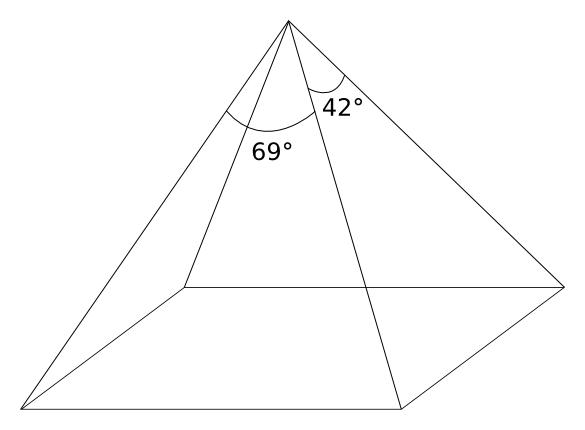
\includegraphics{images/fov.png}
    \caption{Field of view of our webcam.}
    \label{fig:fov}
\end{figure*}

\subsection{Weather}
%% SUNIL

% Loiter mode works well with little wind but struggles when there is heavy wind
% This means that our landing controller oscillates wildly.

\section{Conclusion \& Future Directions}

Use higher quality optics.
Explore landing pad design.
Allow landing in darker scenarios.
Use more advanced control loops (PID instead of just P).
Rewrite roscopter in C++.
Integrate sonar sensor for more accurate altitude estimates.

\printbibliography

\end{document}
